% ============================================================================
%  Appendix: Supplementary Figures and Tables
%  Exhibits moved out of the main body to reduce crowding: the keyword-
%  extraction F1@5 charts, the natural-language-to-IR accuracy table, and the
%  full bi-encoder and cross-encoder score tables. Every \label is preserved,
%  so all \ref cross-references in the main text resolve here.
%
%  Heading uses the dynamic \appendix system (preamble.sty:307): after \appendix
%  in main.tex, \section{Title} auto-prints "Appendix A: Title" and adds the ToC
%  entry, and a \label here resolves to the letter "A" via \ref.
% ============================================================================

% Start the appendix on a fresh page (the bibliography ends mid-page above).
\clearpage
\section{Supplementary Figures and Tables}
\label{app:deferred}

% --- Keyword extraction F1@5 charts (were Figs 4-6 in the main body) ---------
\begin{figure*}[t]
\centering
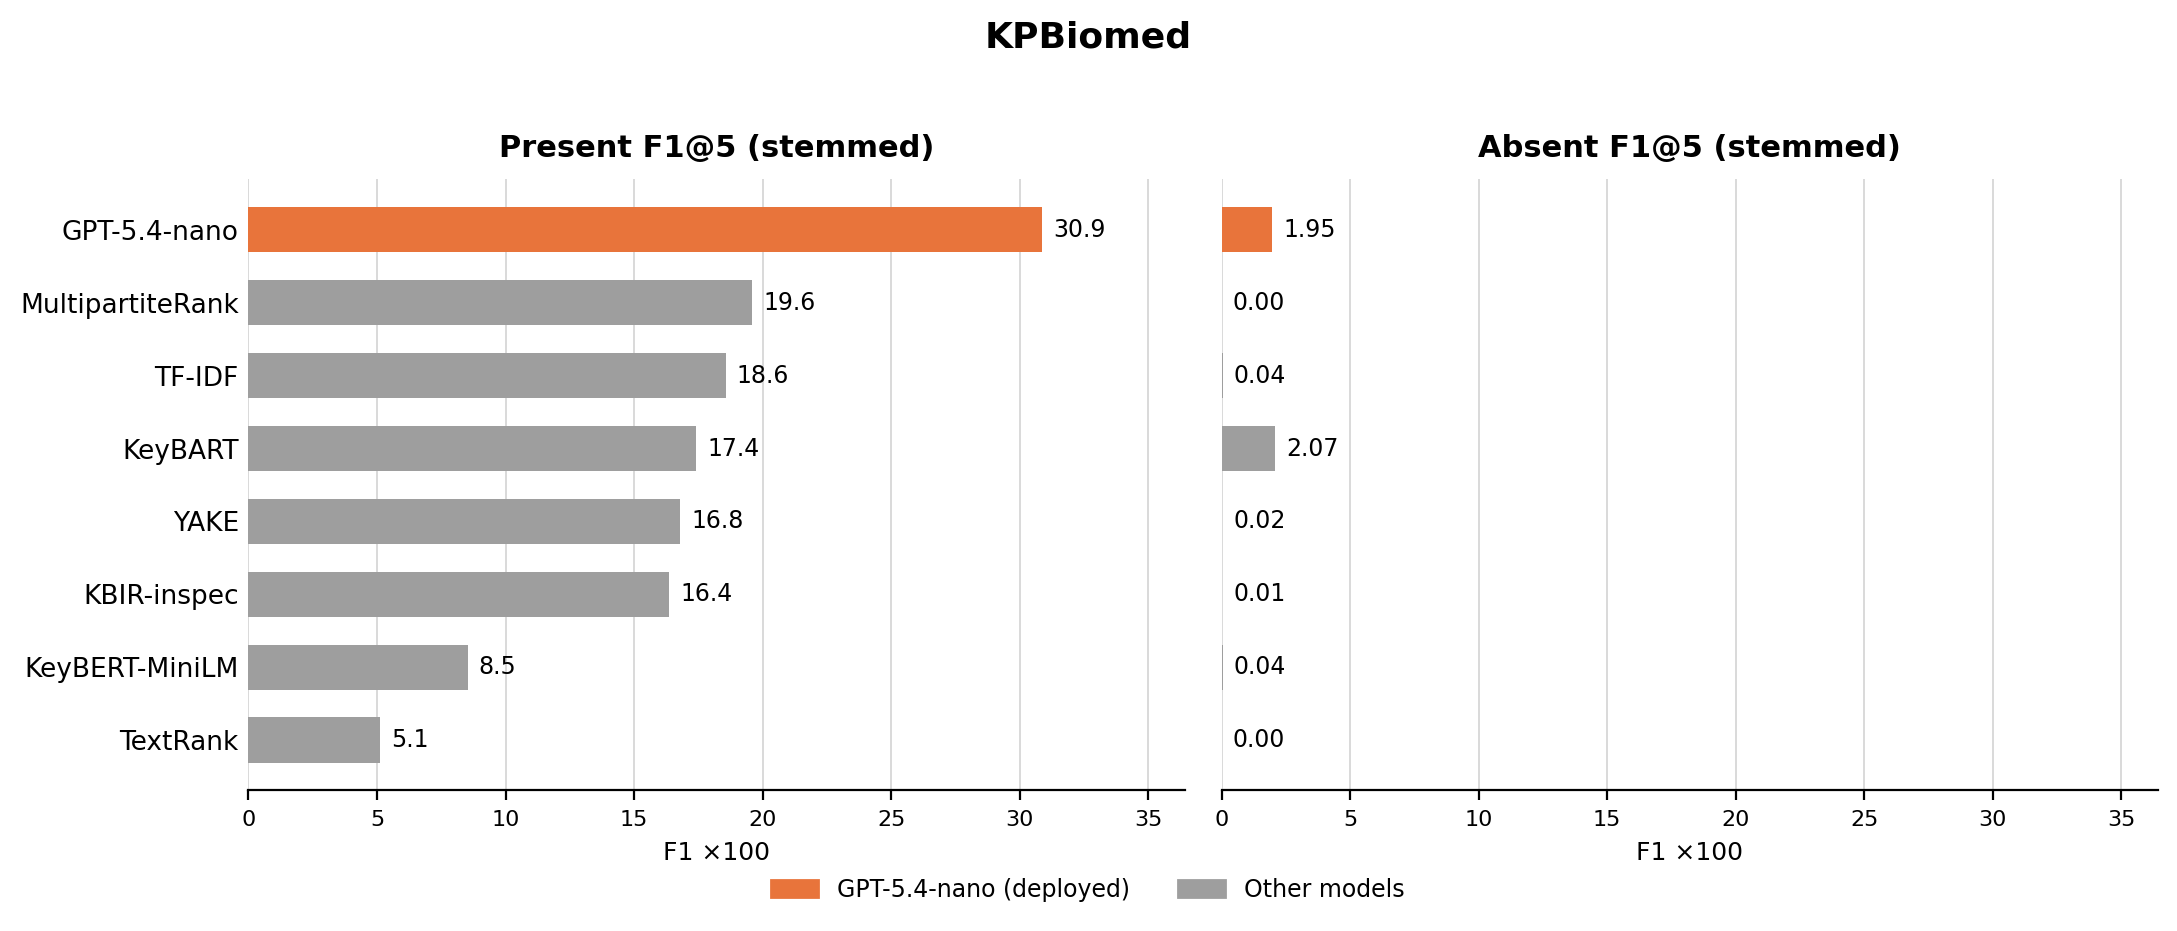
\includegraphics[width=\textwidth]{images/data_and_results/keyword_kpbiomed.png}
\caption{KPBiomed keyword extraction, present and absent F1@5 by model with stemming. The deployed model GPT-5.4-nano is shown in orange and the remaining baselines in grey.}
\label{fig:kw-kpbiomed}
\end{figure*}

\begin{figure*}[t]
\centering
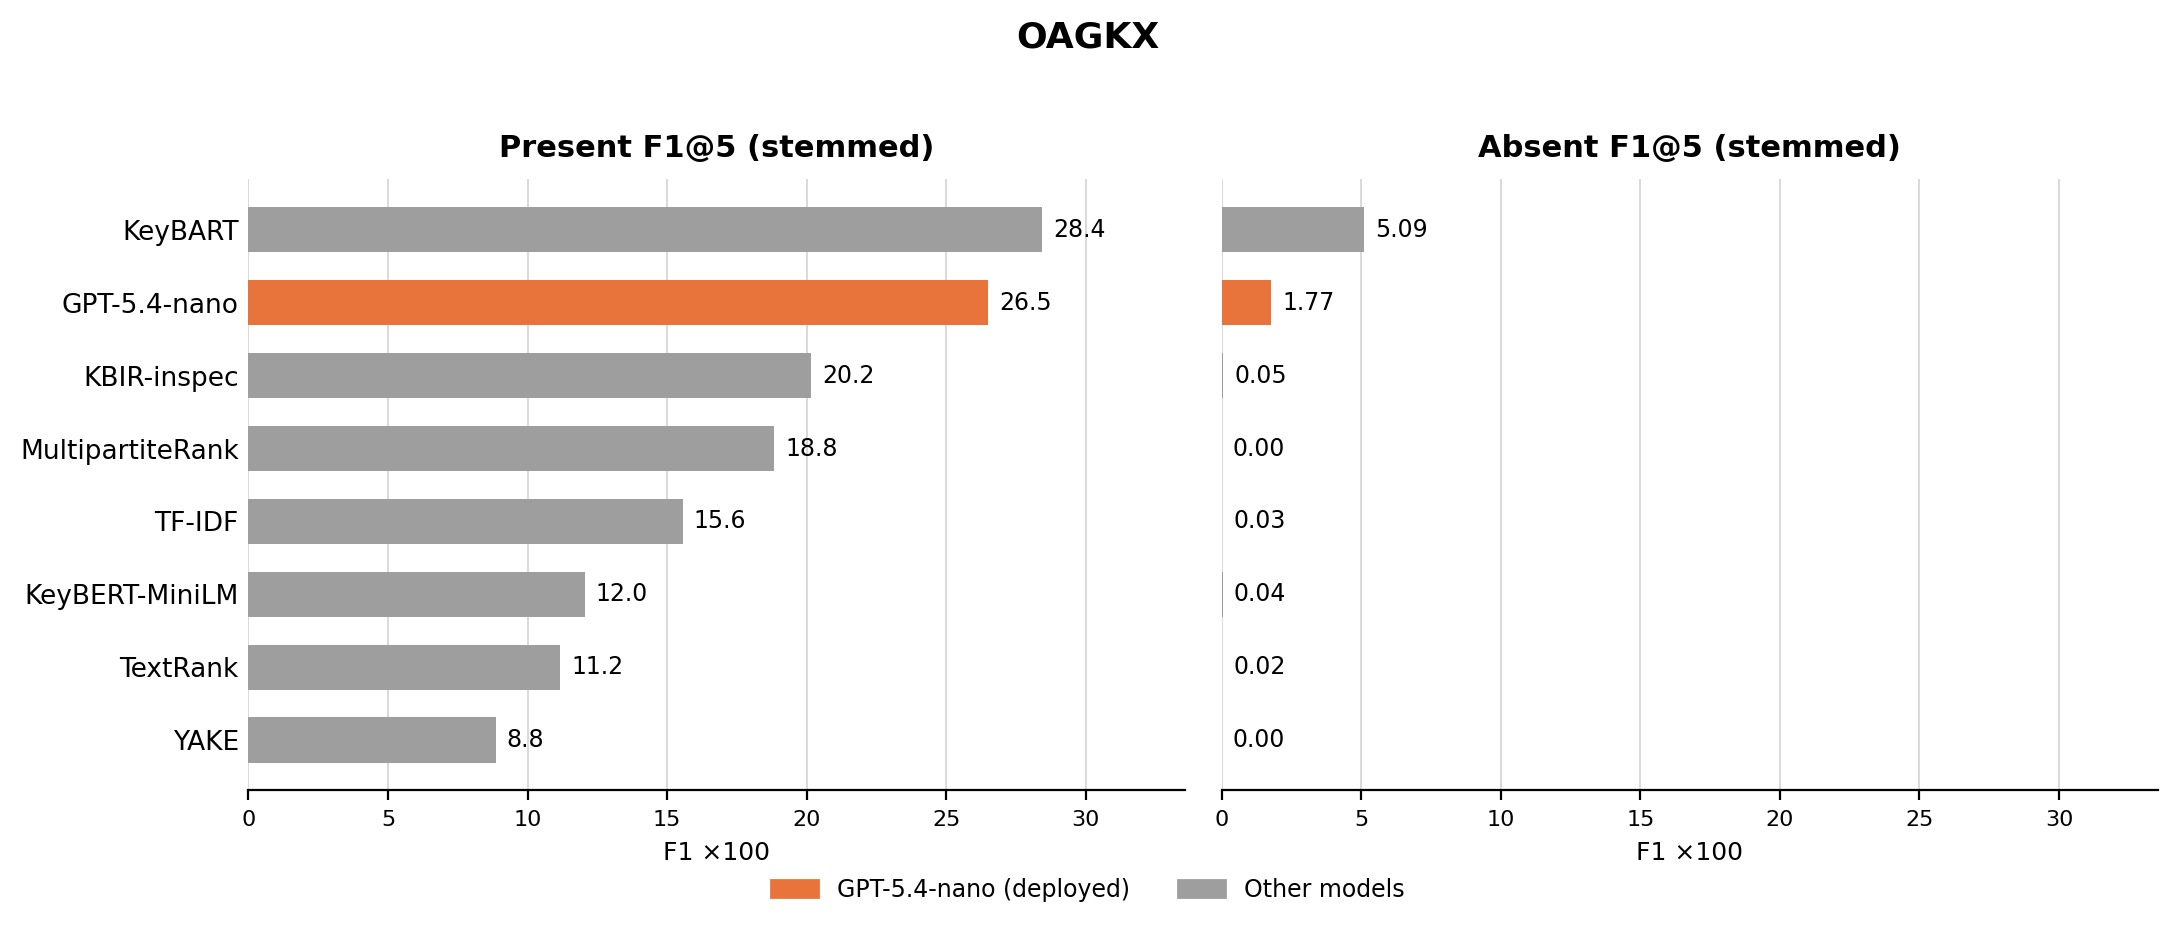
\includegraphics[width=\textwidth]{images/data_and_results/keyword_oagkx.png}
\caption{OAGKX keyword extraction, present and absent F1@5 by model with stemming. The deployed model GPT-5.4-nano is shown in orange and the remaining baselines in grey.}
\label{fig:kw-oagkx}
\end{figure*}

\begin{figure*}[t]
\centering
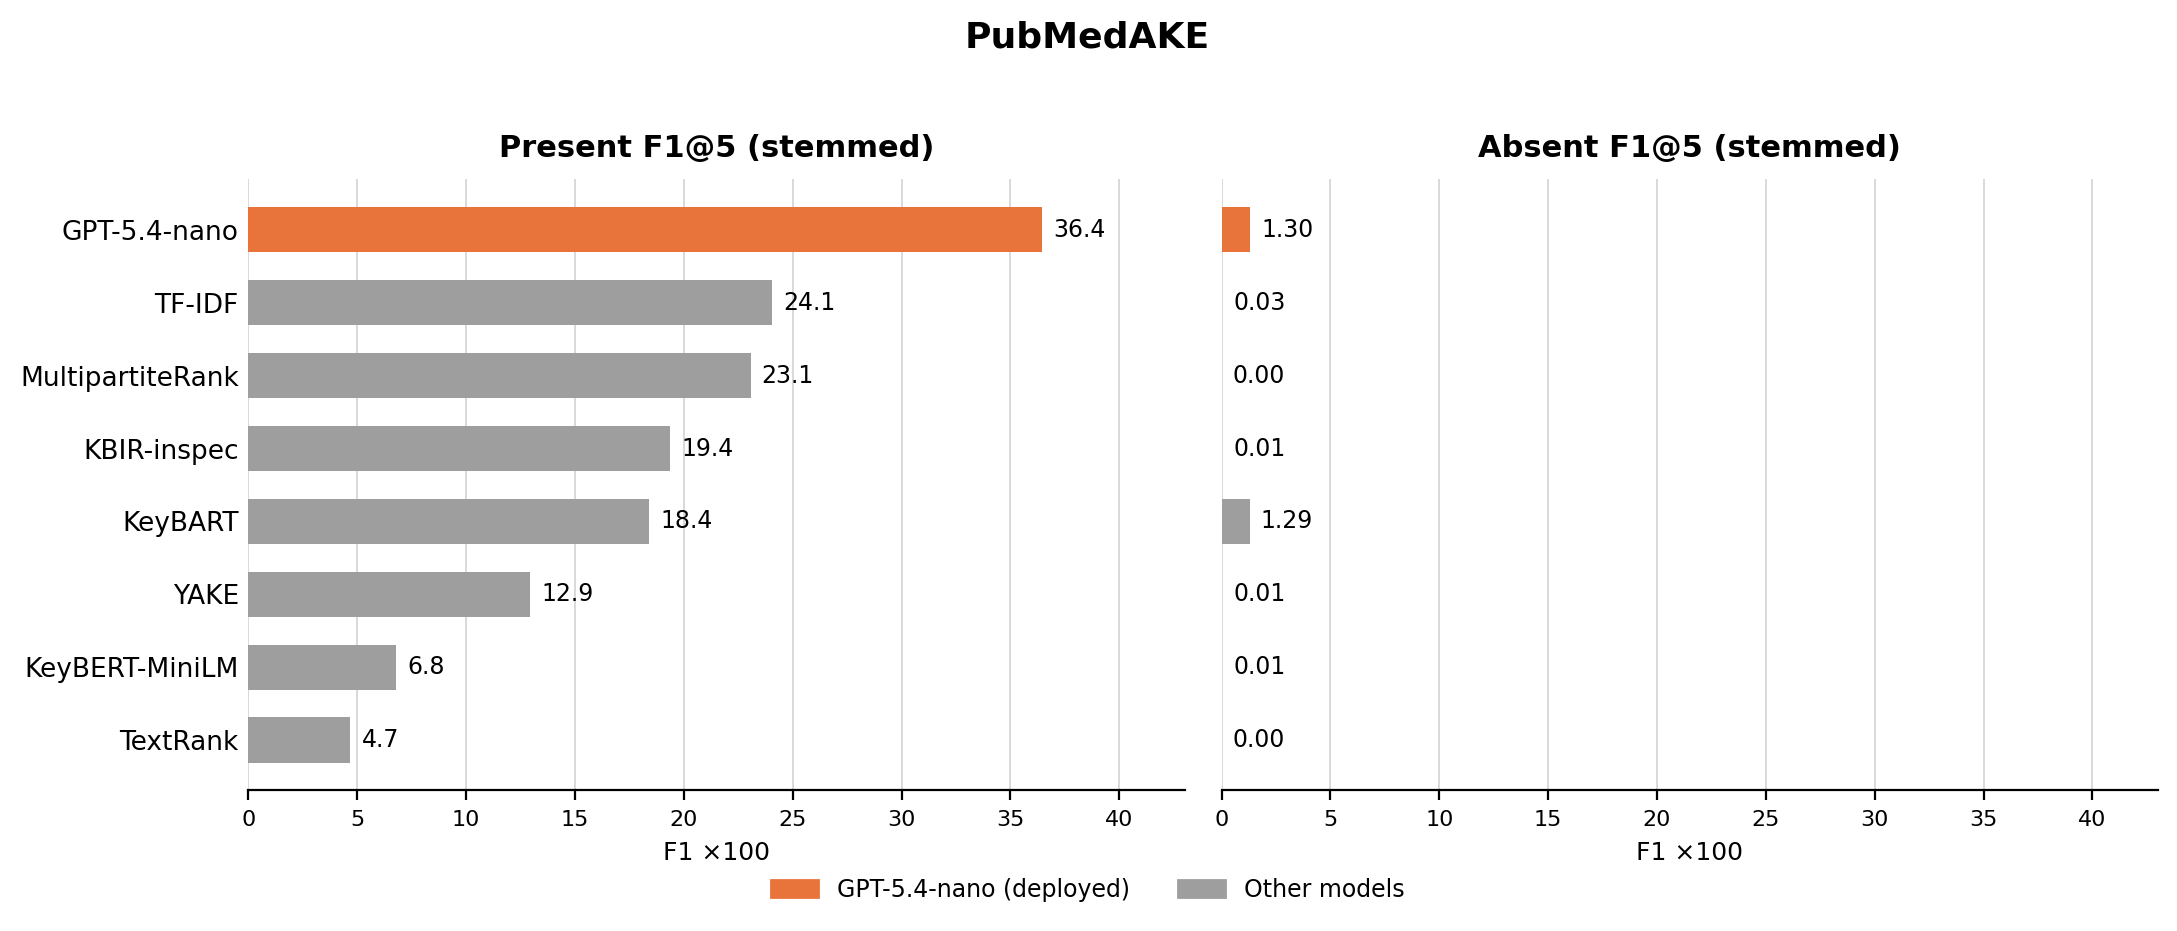
\includegraphics[width=\textwidth]{images/data_and_results/keyword_pubmedake.png}
\caption{PubMedAKE keyword extraction, present and absent F1@5 by model with stemming. The deployed model GPT-5.4-nano is shown in orange and the remaining baselines in grey.}
\label{fig:kw-pubmedake}
\end{figure*}

% --- Natural-language-to-IR accuracy (was Table IX) --------------------------
\begin{table*}[t]
\caption{Natural-language-to-IR accuracy by model. Joint IR accuracy counts a query as correct when both its entities and its Boolean expression are correct under exact matching, reported in the as-deployed or best configuration for each model.}
\label{tab:ir-accuracy}
\centering
\footnotesize
\begin{tabular}{@{}lllcc@{}}
\toprule
Model & Host & Configuration & IR accuracy & 95\% CI \\
\midrule
\textbf{gpt-5.4-nano} & Azure & default, 0 reasoning tok & \textbf{0.937}$^{\dagger}$ & [0.897, 0.983] \\
gpt-5-mini & Azure & default, 384 reasoning tok & 0.931 & [0.879, 0.974] \\
qwen3:8b & Local (Q4) & single-shot & 0.802 & [0.733, 0.871] \\
qwen3:4b & Local (Q4) & thinking$^{\ddagger}$ & 0.784 & [0.707, 0.862] \\
qwen2.5:3b & Local (Q4) & non-reasoning & 0.207 & [0.138, 0.284] \\
phi4-mini & Local (Q4) & non-reasoning & 0.052 & [0.017, 0.095] \\
llama3.2:3b & Local (Q4) & non-reasoning & 0.026 & [0.000, 0.060] \\
\bottomrule
\end{tabular}

\vspace{3pt}
\begin{minipage}{\linewidth}
\footnotesize\itshape
Confidence intervals are 95 percent bootstrap over 1000 iterations. Cross-model gaps that fall within these intervals are treated as ties, and bold marks the deployed model. The dagger denotes a three-run mean, whose single-run range is 0.931 to 0.940, with temperature zero returning a byte-identical output on 96.6 percent of queries (Table~\ref{tab:ir-stability}). The double dagger denotes qwen3:4b, whose single-shot configuration produced degenerate empty output, so its thinking configuration is its only usable score.
\end{minipage}
\end{table*}

% --- Dense bi-encoder full scores (was Table XIV) ---------------------------
\begin{table*}[t]
\caption{Dense bi-encoder retrieval on SciRepEval ad-hoc search, nDCG $\times$100 with 95 percent bootstrap confidence intervals.}
\label{tab:bienc-results}
\centering
\scriptsize
\setlength{\tabcolsep}{4pt}
\begin{tabular}{@{}p{3.0cm}llll@{}}
\toprule
Model & NFCorpus & TREC-CoVID & Search & Average \\
\midrule
Qwen3-Embedding-4B (int8) & \textbf{80.02 [77.75, 82.17]} & \textbf{94.28 [92.96, 95.43]} & 75.54 [74.93, 76.17] & \textbf{83.28 [82.35, 84.19]} \\
EmbeddingGemma-300M & 79.13 [76.84, 81.29] & 92.45 [90.68, 94.03] & 75.32 [74.66, 75.93] & 82.30 [81.32, 83.31] \\
Qwen3-Embedding-0.6B & 77.94 [75.75, 80.22] & 93.90 [92.52, 95.10] & 75.03 [74.41, 75.65] & 82.29 [81.32, 83.25] \\
text-embedding-3-small (existing) & 78.78 [76.61, 81.05] & 92.38 [90.58, 93.96] & 75.14 [74.52, 75.74] & 82.10 [81.08, 83.05] \\
mxbai-embed-large-v1 & 79.37 [77.19, 81.72] & 91.77 [90.02, 93.25] & 74.92 [74.29, 75.56] & 82.02 [81.06, 82.96] \\
SPECTER2-adhoc-query & 70.46 [68.01, 72.97] & 90.08 [87.84, 92.13] & \textbf{78.22 [77.60, 78.86]} & 79.59 [78.46, 80.71] \\
BGE-M3 & 74.05 [71.72, 76.35] & 89.21 [87.08, 91.16] & 74.82 [74.20, 75.46] & 79.36 [78.29, 80.42] \\
SPECTER2-base (existing) & 72.03 [69.60, 74.54] & 89.46 [86.99, 91.58] & 73.76 [73.12, 74.41] & 78.42 [77.27, 79.58] \\
\bottomrule
\end{tabular}

\vspace{3pt}
\begin{minipage}{\linewidth}
\footnotesize\itshape
The metric is SciRepEval ad-hoc-search full-ranking nDCG over a per-query candidate pool, not BEIR full-corpus nDCG@10. Confidence intervals are 95 percent bootstrap [lo, hi] over 1000 iterations with seed 42, and bold marks the best point estimate per column. On Average the top five models' intervals overlap, a statistical tie, and SPECTER2-adhoc-query's Search lead is the one between-model gap whose interval clears the general models.
\end{minipage}
\end{table*}

% --- Cross-encoder full scores (was Table XVI) ------------------------------
\begin{table*}[t]
\caption{Cross-encoder re-ranking on SciRepEval ad-hoc search, nDCG $\times$100 with 95 percent bootstrap confidence intervals, sorted by Average.}
\label{tab:xenc-results}
\centering
\scriptsize
\setlength{\tabcolsep}{4pt}
\begin{tabular}{@{}p{3.2cm}llll@{}}
\toprule
Model (scorer) & NFCorpus & TREC-CoVID & Search & Average \\
\midrule
Cohere Rerank 4.0 Pro (API) & \textbf{80.42 [78.17, 82.60]} & \textbf{94.60 [93.30, 95.71]} & 75.39 [74.76, 76.00] & \textbf{83.47 [82.54, 84.33]} \\
Qwen3-Reranker-4B (int8) & 80.10 [77.94, 82.14] & 94.37 [92.90, 95.60] & 74.93 [74.32, 75.56] & 83.13 [82.18, 83.99] \\
Cohere Rerank 4.0 Fast (API) & 78.77 [76.55, 80.98] & 94.15 [92.83, 95.31] & \textbf{75.42 [74.75, 76.04]} & 82.78 [81.83, 83.68] \\
Qwen3-Reranker-0.6B (fp16) & 78.06 [75.65, 80.24] & 93.98 [92.59, 95.20] & 75.25 [74.59, 75.85] & 82.43 [81.50, 83.34] \\
mxbai-rerank-large-v1 (435M) & 78.32 [76.08, 80.76] & 91.50 [89.43, 93.33] & 74.78 [74.15, 75.46] & 81.53 [80.48, 82.59] \\
jina-reranker-v2-base (278M) & 76.73 [74.49, 79.01] & 91.84 [90.05, 93.52] & 75.37 [74.73, 75.99] & 81.31 [80.28, 82.30] \\
MedCPT-Cross-Encoder (109M, biomed) & 75.70 [73.21, 78.03] & 88.91 [86.61, 90.97] & 73.97 [73.34, 74.63] & 79.53 [78.40, 80.66] \\
ms-marco-MiniLM-L-6-v2 (22M) & 73.10 [70.78, 75.48] & 88.78 [86.41, 90.90] & 75.21 [74.58, 75.84] & 79.03 [77.90, 80.13] \\
bge-reranker-v2-m3 (568M) & 70.71 [68.31, 73.07] & 90.30 [88.29, 92.18] & 74.40 [73.78, 75.05] & 78.47 [77.37, 79.53] \\
ms-marco-MiniLM-L-12-v2 (33M) & 69.88 [67.41, 72.38] & 87.17 [84.73, 89.52] & 75.09 [74.44, 75.71] & 77.38 [76.17, 78.54] \\
bge-reranker-large (560M) & 66.49 [64.11, 68.85] & 87.27 [84.61, 89.62] & 74.22 [73.59, 74.85] & 76.00 [74.80, 77.16] \\
bge-reranker-base (278M) & 58.75 [56.38, 60.94] & 84.98 [82.12, 87.60] & 72.60 [71.97, 73.24] & 72.11 [70.84, 73.35] \\
gte-reranker-modernbert-base (150M) & 48.88 [46.82, 50.93] & 79.03 [76.40, 81.60] & 69.94 [69.26, 70.60] & 65.95 [64.91, 67.07] \\
\bottomrule
\end{tabular}

\vspace{3pt}
\begin{minipage}{\linewidth}
\footnotesize\itshape
The metric is SciRepEval ad-hoc-search full-ranking nDCG over a reranking pool, not BEIR full-corpus nDCG@10. Confidence intervals are 95 percent bootstrap [2.5 percent, 97.5 percent] over 1000 iterations with seed 42, with the Average resampled independently within each dataset. The intervals are tight on Search, which has 2585 queries, and wide on TREC-CoVID, which has 50, and bold marks the best point estimate per column. The top four models, namely Cohere Pro, Qwen3-Reranker-4B, Cohere Fast, and Qwen3-Reranker-0.6B, have heavily overlapping Average intervals and form a statistical tie, within which the best self-hostable model, Qwen3-Reranker-4B at int8, is tied with Cohere Pro. On Search the small candidate pool saturates every reranker at around 75. For reference, the bi-encoder embeddings without intervals give the best embedder Qwen3-Embedding-4B at 83.28 Average, SPECTER2-adhoc-query at 78.22 on Search, which is above every reranker here, and text-embedding-3-small at 82.10 Average.
\end{minipage}
\end{table*}

% Flush all appendix floats before the document ends / any column-mode change.
\clearpage